\section{Online-Farm status}

%\begin{frame}{The main event data model}{}
%	\begin{center} 
%		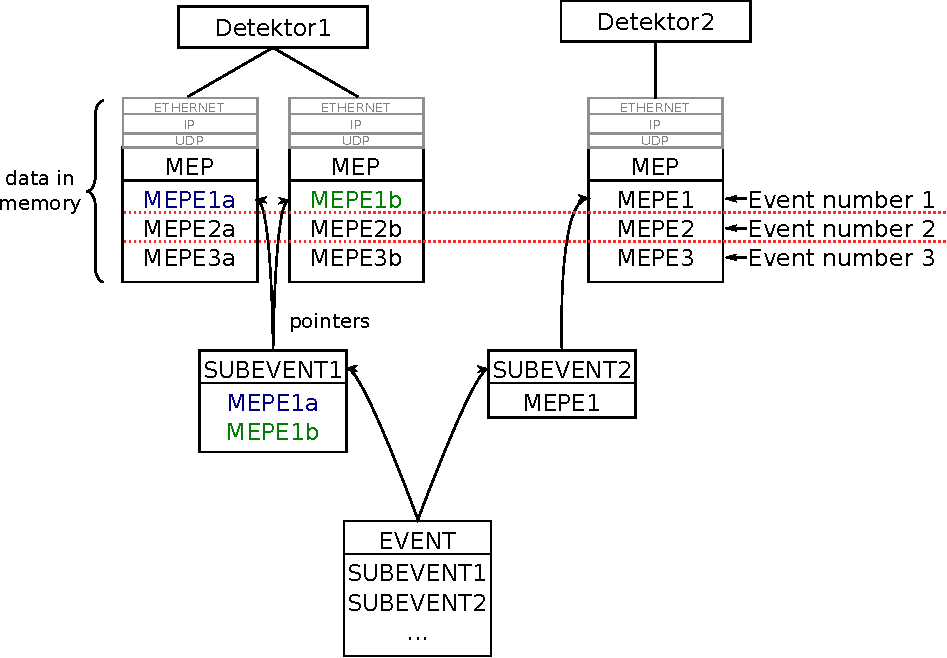
\includegraphics[width=8cm]{eb-data-model}
%	\end{center} 
%\end{frame}

\begin{frame}[plain]{Farm - Data flow overview}{}
	\begin{center} 
		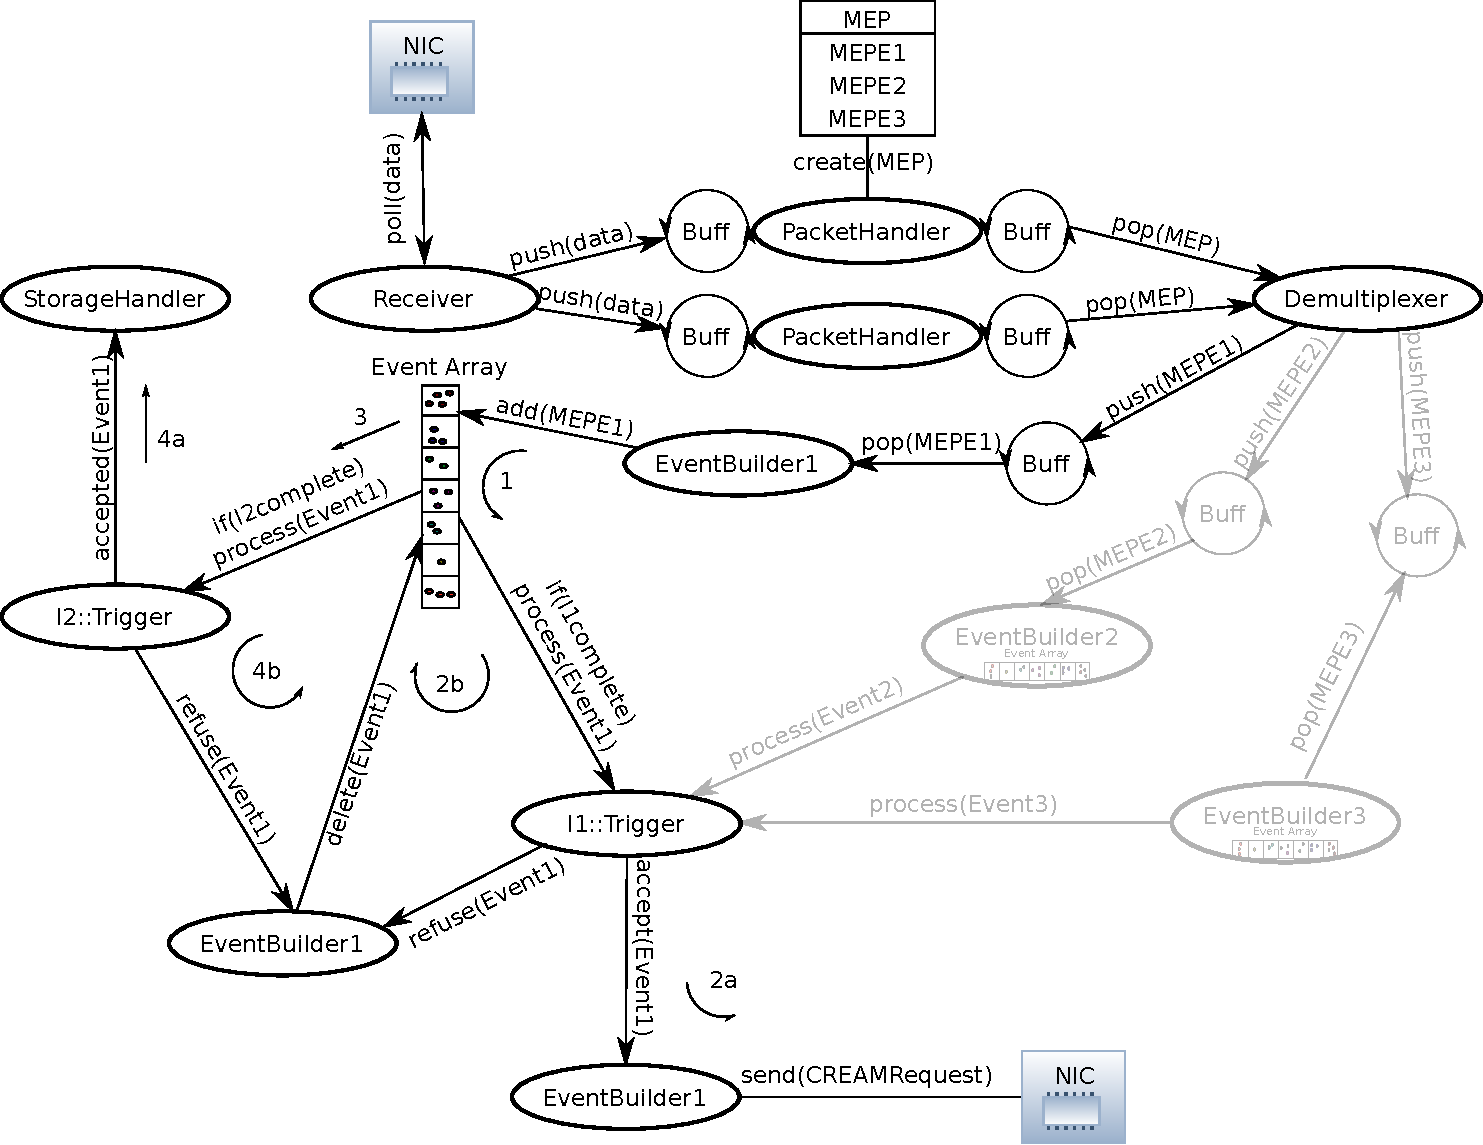
\includegraphics[width=\textwidth]{farm-concept}
	\end{center} 
\end{frame}

%\begin{frame}[fragile]
%\frametitle{Event building}
%\begin{lstlisting}[frame=trBL,caption={}]{hallowelt}
%EBs[mepEvent%EBNUM]->add(mepEvent);
%void EB::add(MEPEvent* mepEvent){
%    Event* event = eventPool[mepEvent->getEventNumber()/EBNUM];
%    if(event->addPacket(mepEvent)){
%        if(event->L1Processed()){
%           if(L2T->Process(event))
%                DataHandler->send(event);
%           event->destroy();
%        } else {
%           if(!L1T->Process(event))
%               event->destroy();
%        }
%    }
%}
%\end{lstlisting}
%\end{frame}

\begin{frame}{Summary}{}
	\begin{block}{Done so far}
		\begin{itemize}
		  \item Receiving L0-Data as defined in note NA62-11-02
		  \item Integrity checks (Packet sizes, event numbers)
		  \item L1-Eventbuilding
		  \item Basic interface for L1 trigger software (any proposal?)
		\end{itemize}
	\end{block}
	
	\begin{block}{Missing}
		\begin{itemize}
	  		\item IP CRC check (can we let the NIC do that?)
	  		\item CREAM data request
	  		\item Interface for L2 trigger software
	  		\item Interface to storage/tapes
	  		\item Monitoring frontend (any ideas?)
		\end{itemize}
	\end{block}
\end{frame}

\begin{frame}{Load (very first rough estimation)}{}

Full Speed L1 simulation:
\begin{itemize}
  \item about 900kHz MEP rate
  \item 3 Events per MEP, 450B each
  \item 10 Detektors
  \item $\Rightarrow$ about 270kHz Event rate 
\end{itemize}

\begin{table}
	\begin{tabular}{c c c}
		Process	& Threads	& CPU Load \\
		\hline
		Receiver		&	1	&	100\% \\
		PacketHandler	&	2	&	$\approx180$\% \\
		EventBuilder	&	22	&	$\approx$300\%	\\
		L1 SUM	&	22	&	$\approx$1200\%
	\end{tabular}
	\end{table}
	\begin{ergo}
		About 18 cores remaining for L1 and L2 Trigger processing
	\end{ergo}
\end{frame}


%\begin{frame}{Monitoring the Farm}{}
%	\begin{center} 
%		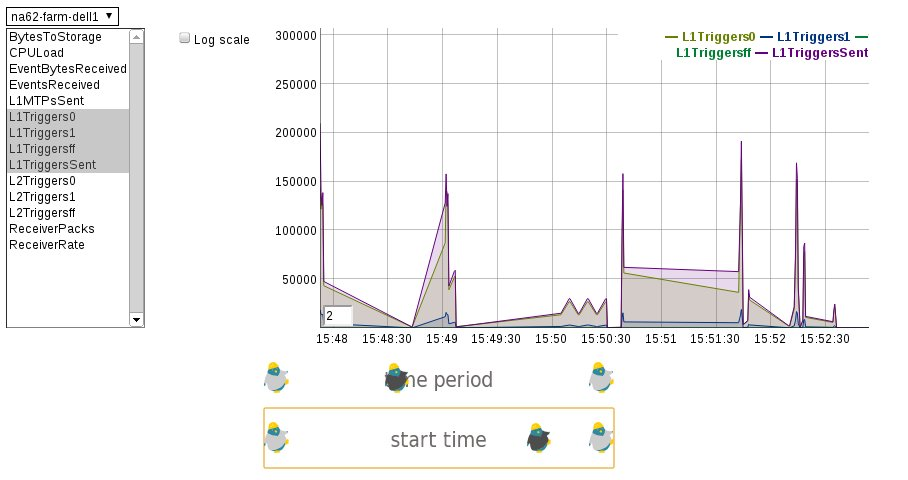
\includegraphics[width=0.7\textwidth]{monitoring}
%	\end{center}
%	\begin{itemize}
%	  \item What DB? MySQL?!
%	  \item What rate? 1-second average?!
%	  \item How to visualize? GWT?! rrd-Based tools like OPS/ganglia only allow
%	  1-min average.
%	\end{itemize}
%\end{frame}